% \begin{table}[t]
% \centering
% \ra{1.2}
% \caption{Statistics of dependency graphs generated for the 15 attacks}
% \label{tab:rq1}
% \resizebox{0.48\textwidth}{!}{
% \begin{tabular}{@{}crrrrr@{}}
% \toprule
% \textbf{Attack}      & \multicolumn{1}{c}{\textbf{CPR}} & \multicolumn{1}{c}{\textbf{ReadOnly}} & \multicolumn{1}{c}{\textbf{PrioTracker}} & \multicolumn{1}{c}{\textbf{NoDoze}} & \multicolumn{1}{c}{\textbf{\tool}} \\ \midrule
% Wget Executable      & 363                           & 58                                 & 58                                    & 288                              & 48                                \\
% Illegal Storage      & 62,073                        & 16,211                             & 6,948                                 & 10,260                           & 43                                \\
% Illegal Storage2     & 378,326                       & 89,779                             & 37,112                                & 19,512                           & 7                                 \\
% Hide File            & 3,273,769                     & 613,303                            & 114,614                               & 37,251                           & 437                               \\
% Steal Information    & 3,291,208                     & 618,025                            & 115,223                               & 20,426                           & 750                               \\
% Backdoor Download    & 60,390                        & 15,990                             & 6,024                                 & 269                              & 20                                \\
% Annoying Server User & 318                           & 56                                 & 39                                    & 227                              & 23                                \\
% Shellshcok           & 3,600                         & 590                                & 518                                   & 911                              & 451                               \\
% Dataleak             & 1,152                         & 231                                & 211                                   & 687                              & 223                               \\
% VPN Filter           & 1,879                         & 298                                & 244                                   & 217                              & 263                               \\
% Five Dir. Case1      & 272                           & 18                                 & 18                                    & 257                              & 7                                 \\
% Five Dir. Case3      & 78,075                        & 77,824                             & 7,496                                 & 598                              & 33                                \\
% Theia Case1          & 816,277                       & 325,459                            & 176,800                               & 151,240                          & 62                                \\
% Theia Case3          & 1,500,717                     & 537,424                            & 269,277                               & 9,015                            & 10                                \\
% Trace Case5          & 971                           & 910                                & 459                                   & 510                              & 4                                 \\
% \textbf{AVG}         & 631,292.67                       & 153,078.40                            & 49,002.73                                & 16,777.87                           & 158.73                               \\ \bottomrule
% \end{tabular}
% }
% \end{table}



\begin{table*}[t]
\centering
\ra{1.2}
\caption{Dependency graphs generated by each technique}
\label{tab:rq1}
\resizebox{\textwidth}{!}{
\begin{tabular}{c|rrr|rrr|rrr|rrr|rrr}
\hline
\multirow{2}{*}{\textbf{Attack}}      & \multicolumn{1}{c}{\textbf{}}               & \multicolumn{1}{c}{\textbf{CPR}}            & \multicolumn{1}{c|}{\textbf{}}            & \multicolumn{1}{c}{\textbf{}}               & \multicolumn{1}{c}{\textbf{ReadOnly}}       & \multicolumn{1}{c|}{\textbf{}}            & \multicolumn{1}{c}{\textbf{}}               & \multicolumn{1}{c}{\textbf{Priotracker}}    & \multicolumn{1}{c|}{\textbf{}}            & \multicolumn{1}{c}{\textbf{}}               & \multicolumn{1}{c}{\textbf{NoDoze}}         & \multicolumn{1}{c|}{\textbf{}}            & \multicolumn{1}{c}{\textbf{}}               & \multicolumn{1}{c}{\textbf{DepImpact}}      & \multicolumn{1}{c}{\textbf{}}            \\
\textbf{}            & \multicolumn{1}{c}{\textbf{FP}} & \multicolumn{1}{c}{\textbf{FN}} & \multicolumn{1}{c|}{\textbf{\# Edges}} & \multicolumn{1}{c}{\textbf{FP}} & \multicolumn{1}{c}{\textbf{FN}} & \multicolumn{1}{c|}{\textbf{\# Edges}} & \multicolumn{1}{c}{\textbf{FP}} & \multicolumn{1}{c}{\textbf{FN}} & \multicolumn{1}{c|}{\textbf{\# Edges}} & \multicolumn{1}{c}{\textbf{FP}} & \multicolumn{1}{c}{\textbf{FN}} & \multicolumn{1}{c|}{\textbf{\# Edges}} & \multicolumn{1}{c}{\textbf{FP}} & \multicolumn{1}{c}{\textbf{FN}} & \multicolumn{1}{c}{\textbf{\# Edges}} \\ \hline
Wget Executable      & 355                                         & 0                                           & 363                                       & 50                                          & 0                                           & 58                                        & 50                                          & 0                                           & 58                                        & 283                                         & 3                                           & 288                                       & 45                                          & 0                                           & 53                                       \\
Illegal Storage      & 62067                                       & 0                                           & 62073                                     & 16206                                       & 1                                           & 16211                                     & 6943                                        & 1                                           & 6948                                      & 10254                                       & 0                                           & 10260                                     & 71                                          & 0                                           & 77                                       \\
Illegal Storage2     & 378322                                      & 0                                           & 378326                                    & 89775                                       & 0                                           & 89779                                     & 37108                                       & 0                                           & 37112                                     & 19509                                       & 1                                           & 19512                                     & 624                                         & 0                                           & 628                                      \\
Hide File            & 3273757                                     & 0                                           & 3273769                                   & 613294                                      & 3                                           & 613303                                    & 114604                                      & 2                                           & 114614                                    & 37241                                       & 2                                           & 37251                                     & 797                                         & 0                                           & 809                                      \\
Steal Information    & 3291204                                     & 0                                           & 3291208                                   & 618021                                      & 0                                           & 618025                                    & 115219                                      & 0                                           & 115223                                    & 20423                                       & 1                                           & 20426                                     & 854                                         & 0                                           & 858                                      \\
Backdoor Download    & 60382                                       & 0                                           & 60390                                     & 15982                                       & 0                                           & 15990                                     & 6017                                        & 1                                           & 6024                                      & 261                                         & 0                                           & 269                                       & 121                                         & 0                                           & 129                                      \\
Annoying Server User & 308                                         & 0                                           & 318                                       & 46                                          & 0                                           & 56                                        & 31                                          & 2                                           & 39                                        & 219                                         & 2                                           & 227                                       & 14                                          & 0                                           & 24                                       \\
Shellshcok           & 3570                                        & 0                                           & 3600                                      & 577                                         & 17                                          & 590                                       & 493                                         & 5                                           & 518                                       & 885                                         & 4                                           & 911                                       & 444                                         & 0                                           & 474                                      \\
Dataleak             & 1134                                        & 0                                           & 1152                                      & 220                                         & 7                                           & 231                                       & 199                                         & 6                                           & 211                                       & 673                                         & 4                                           & 687                                       & 214                                         & 0                                           & 232                                      \\
VPN Filter           & 1869                                        & 0                                           & 1879                                      & 290                                         & 2                                           & 298                                       & 238                                         & 4                                           & 244                                       & 208                                         & 1                                           & 217                                       & 59                                          & 0                                           & 69                                       \\
Five Dir Case1       & 270                                         & 0                                           & 272                                       & 17                                          & 1                                           & 18                                        & 17                                          & 1                                           & 18                                        & 255                                         & 0                                           & 257                                       & 8                                           & 0                                           & 10                                       \\
Five Dir Case3       & 78071                                       & 0                                           & 78075                                     & 77824                                       & 4                                           & 77824                                     & 7493                                        & 1                                           & 7496                                      & 595                                         & 1                                           & 598                                       & 29                                          & 0                                           & 33                                       \\
Theia Case1          & 816269                                      & 0                                           & 816277                                    & 325459                                      & 8                                           & 325459                                    & 176794                                      & 2                                           & 176800                                    & 151233                                      & 1                                           & 151240                                    & 54                                          & 0                                           & 62                                       \\
Theia Case3          & 1500711                                     & 0                                           & 1500717                                   & 537424                                      & 6                                           & 537424                                    & 269274                                      & 3                                           & 269277                                    & 9010                                        & 1                                           & 9015                                      & 46                                          & 0                                           & 52                                       \\
Trace Case5          & 968                                         & 0                                           & 971                                       & 910                                         & 3                                           & 910                                       & 458                                         & 2                                           & 459                                       & 509                                         & 2                                           & 510                                       & 1                                           & 0                                           & 4                                        \\
\textbf{AVG}         & 631283.80                                   & 0.00                                        & 631292.67                                 & 153073.00                                   & 3.47                                        & 153078.40                                 & 48995.87                                    & 2.00                                        & 49002.73                                  & 16770.53                                    & 1.53                                        & 16777.87                                  & 225.40                                      & 0.00                                        & 234.27                                   \\ \hline
\end{tabular}
}
\end{table*}






\subsection{RQ1: Revealing Attack Sequences}
\label{subsec:rq1}
To demonstrate the effectiveness of \tool in revealing the attack sequence by pruning non-critical edges, we compare \tool with 4 state-of-the-art techniques: CPR~\cite{reduction}, ReadOnly~\cite{loggc}, PrioTracker~\cite{liu2018priotracker}, and NoDoze~\cite{hassan2019nodoze}. 
%As discussed in \cref{subsubsec:entry-ranking},
\tool uses 6 entry nodes, composed of the top 2 entry nodes from the 3 types of system entities (\ie files, processes, and network connections), to perform forward causality analysis, which is shown to preserve all the critical edges (see \cref{subsec:rq2}).
For the attacks involving multiple POI events, we applied \tool on each of the POI events and then union the generated critical components. 
CPR merges edges between two nodes if the time differences between the edges are within a threshold (\ie 10 seconds).
ReadOnly removes the edge whose source node is the read-only file. 
PrioTracker mainly uses the fanout of nodes to prioritize the dependencies in the causality analysis. 
We then adapt the computed priories as the dependency weights for edges and filter the edges with low weights.
%for comparison with \tool. 
NoDoze assigns an anomaly score for each edge based on the frequency of the corresponding system event, and then computes the anomaly score for each path. 
% Paths having higher anomaly scores will be reported. 
As NoDoze requires an execute profile, we use the daily log file of the deployed system as the execution profile for the attacks in our deployed hosts,
and use the normal events in the logs (except the events whose observed time are within the attack period) for the attacks in the DARPA TC dataset.
Based on the ground truth of each attack, we manually assign lower reputation scores for the malicious files and IP addresses as required by NoDoze.
Once NoDoze finishes computing the anomaly scores for the whole graph, we perform the graph reduction based on the anomaly score of each path in the dependency graph. 
% Note that it is fairly easy for a technique to keep all the critical edges by keeping all the edges generated by the causality analysis from the POI event, but it is far more difficult to preserve the critical edges and filter the non-critical edges at the same time. 
% Thus, we tune the parameters of all the techniques to preserve all the critical edges whenever possible, and compare the results of dependency graph reduction in terms of the number of edges.

\cref{tab:rq1} shows the dependency graph reduction of \tool and the other techniques.
The results show that \tool achieves the best performance for dependency graph reduction. 
On average, the size of the dependency graph generated by \tool (\ie the critical component output by \tool) is \emph{at least $106\times$ smaller than the second-best result} (\ie NoDoze) and three or four orders of magnitudes smaller than the other 3 techniques.
We next explain the comparison with each technique.

CPR merges only the edges between pairs of nodes, and thus lack the capabilities to prune irrelevant edges originated from irrelevant system activities.
% the results demonstrate the better pruning power brought by the forward causality analysis from the top-ranked entry nodes.
Removing read-only files is heuristics-based and cannot robustly achieve good performance for different attacks as illustrated by the results (\eg $58$ for the ``Wget executable'' attack v.s. $600,000+$ for the ``Hide File'' attack).
%pure data amount 
% We also try another similar heuristic-based technique that only keeps edges has similar data amount as the POI. But this technique cannot work well for the case whose dependency graph is large. 
% Because for a large dependency graph, many edges have similar data amount, the technique that depends on the simple heuristic rule usually cannot work robustly for real complex attacks.   
The comparison with PrioTracker shows the superiority of our \textit{discriminative feature projection scheme} over the fanout feature in PrioTracker.
From the results, we can observe that NoDoze  performs generally well but poorly for certain attacks (\eg producing graphs with $>10,000$ edges for 5 attacks)
% , \eg the ``Hide File'' attack, the ``Steal information'' attack, and ``Theia Case1'' whose dependency graphs have more than millions of edges. 
The major reason is that there are many rare benign events in these dependency graphs that do not appear in the execution profiles.
% In NoDoze, the anomaly score of a given path is the product of each event's probability along the path. 
% These rare benign events cause many paths that include these benign events to have higher anomaly scores, which greatly degrades the effectiveness of NoDoze.
In other words, the effectiveness of NoDoze heavily relies on whether the execution profile can capture all the benign events, which is generally difficult since the runtime environment of most organizations are dynamic and versatile.
%
On the other hand, compared to NoDoze, \tool achieves better reduction results without sharing its two major limitations:
(1) \tool does not rely on third-party services to assign reputations to malicious files or IP addresses, which may introduce additional risks and complexity;
(2) \tool does not require the execution profile of the deployed system for training. 
These characteristics greatly reduce the difficulty of deploying \tool in a new system, enabling \tool to achieve better generalization than NoDoze.

\begin{figure}[t]
    \centering
    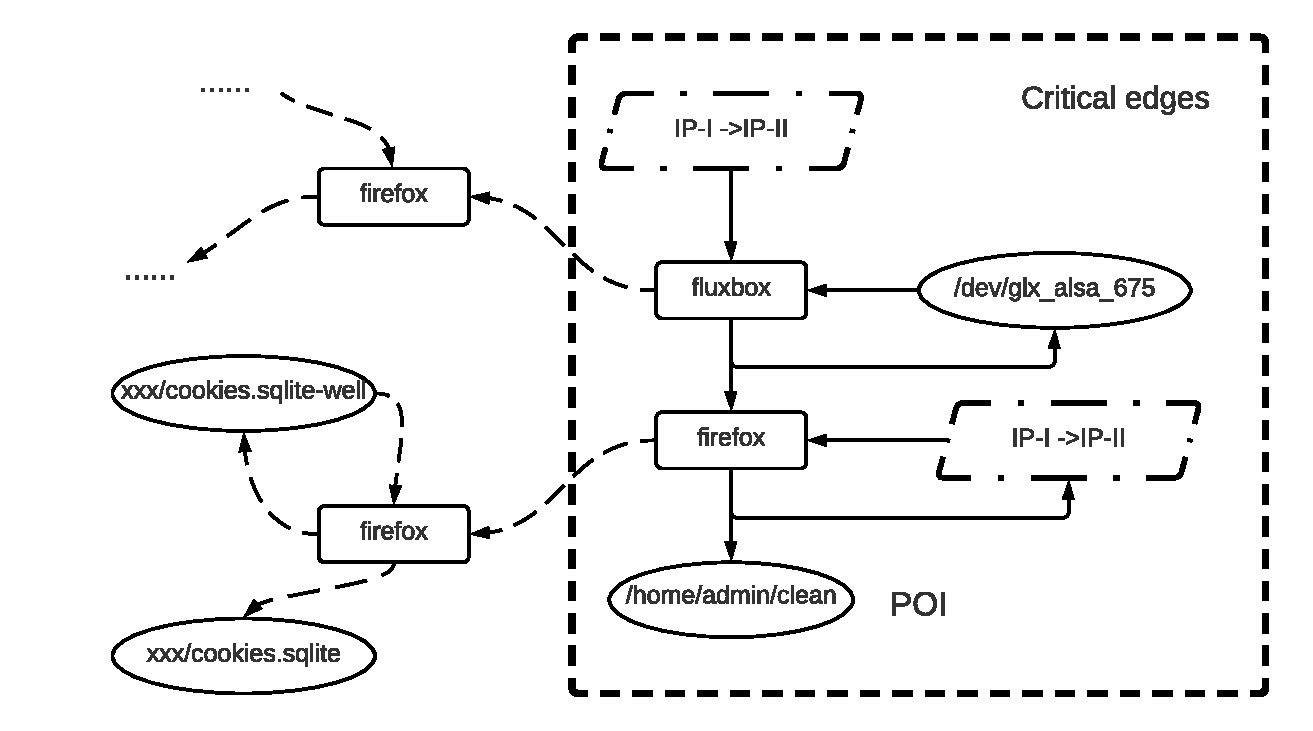
\includegraphics[width=0.47\textwidth]{figs/2021usenix/darpa.pdf}
    \caption{Critical component generated by \tool for the ``Theia Case 1'' attack}
    \label{fig:darpa}
\end{figure} 
\begin{figure*}[t]
    \centering
    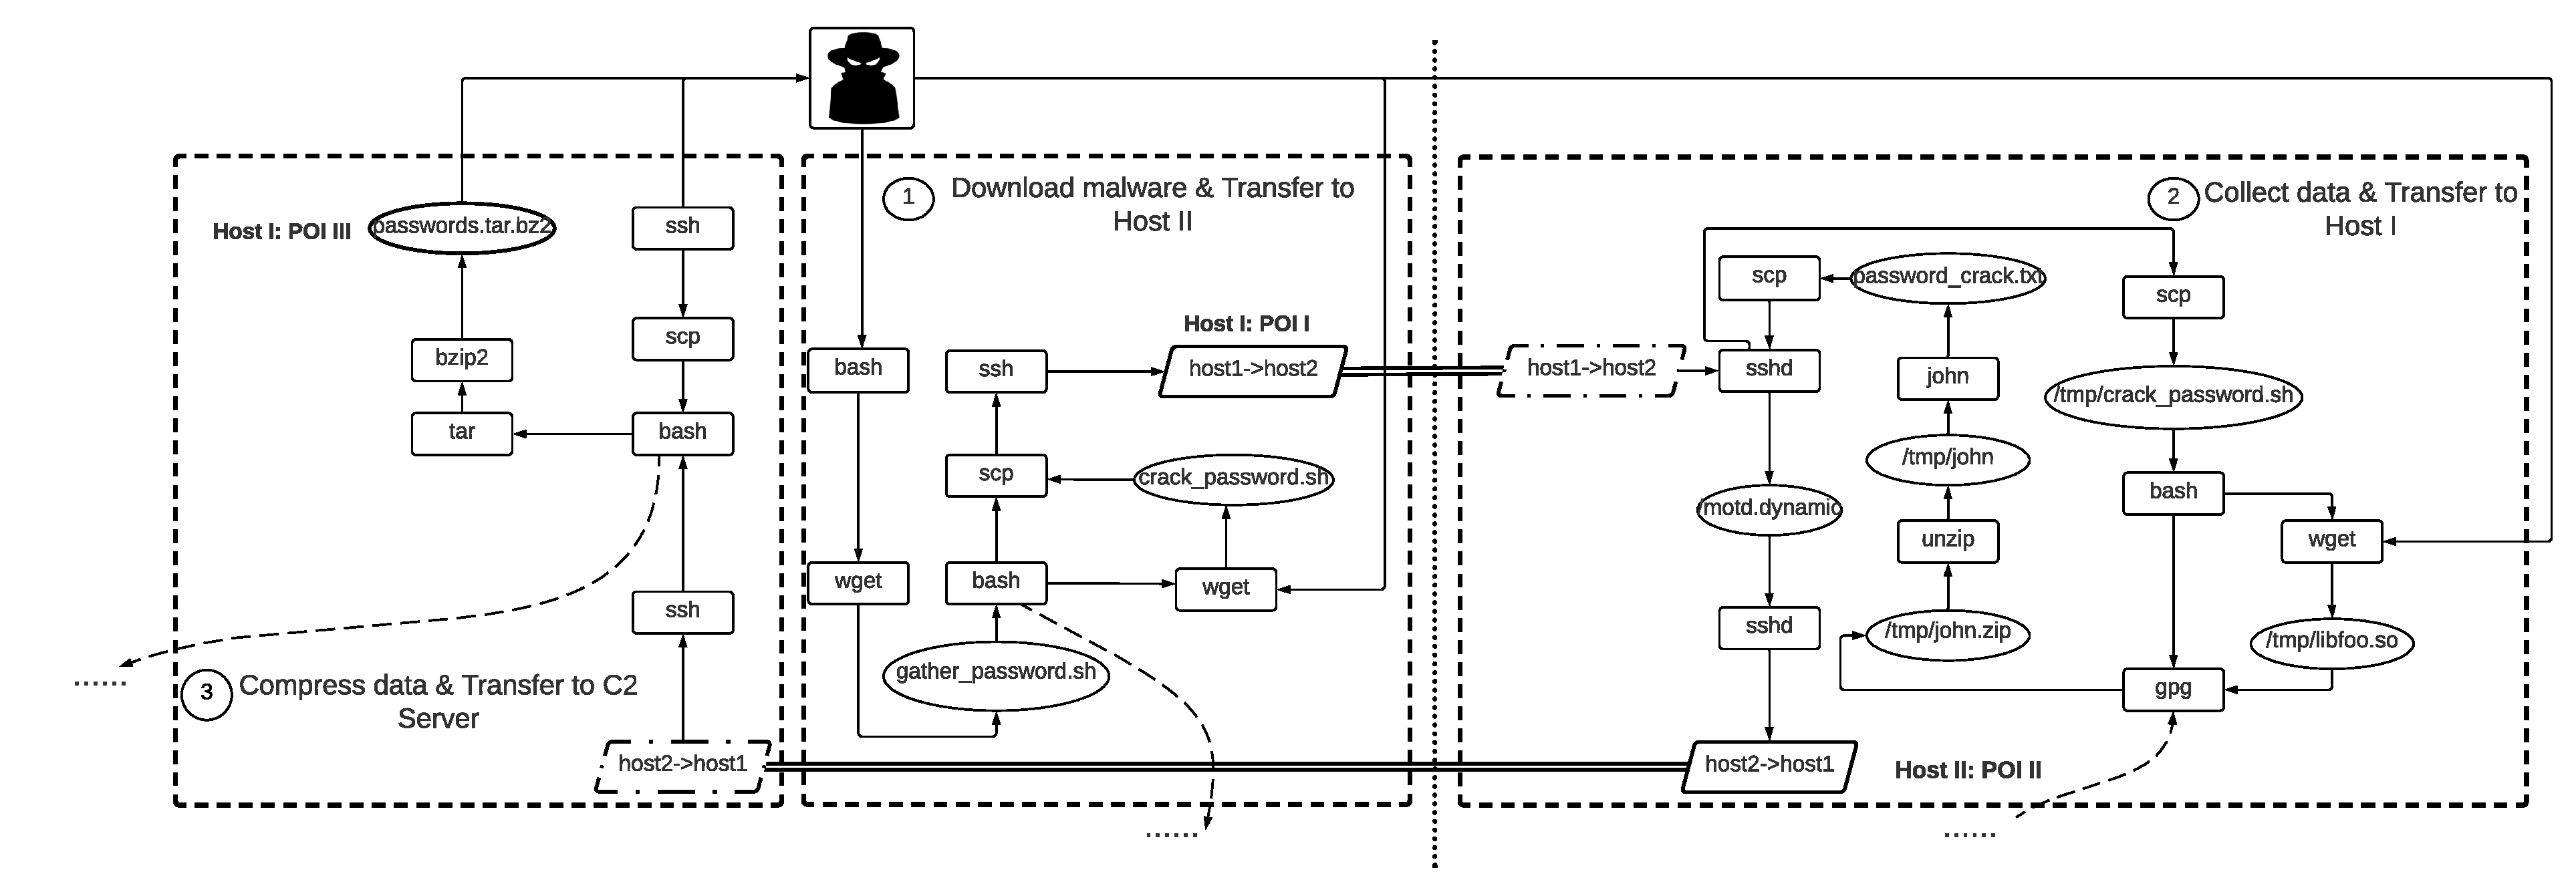
\includegraphics[width=0.9\textwidth, clip]{figs/2021usenix/multihost.pdf}
    \caption{Critical components generated by \tool for the ``Shellshock'' attack (non-critical edges are omitted). \tool generates critical components for the three POI events and takes the union of the generated critical components, which covers all the attack steps as described in \cref{subsubsec:attack-cases}.}
    \label{fig:multi}
\end{figure*}

\myparatight{Case Study}
\cref{fig:darpa,fig:multi} show the critical components of two attacks. 
We use solid lines to represent critical edges, dash lines to represent non-critical edges, and dot-and-dash lines to label attack entries. 
POI events are clearly marked with text descriptions.
% For the POI of the attack, we label the node with text (\ie POI).

\cref{fig:darpa} shows the
%dependency graph 
critical component generated by \tool for the ``Theia Case 1'' attack in the DARPA TC dataset. 
We can observe that the firefox browser is started to download the file \incode{/home/admin/clean} from a malicious IP address.
% which is a backdoor-download behavior. 
Here, the IP addresses (\ie the source of the backdoor) are correctly identified as attack entries, and all the critical edges are preserved.
% The attack entries are the IP addresses, the source of the backdoor.
% The POI is the downloaded file. 
% For this attack, the attack sequence consists of 8 edges and \tool generates a graph of 62 edges that preserves all the 8 edges, while the other state-of-art techniques keep hundreds of thousands of edges, demonstrating the superiority of \tool.



%  POI-I and then get the first critical component, which reflects the attacker downloaded the malicious script and then sent it to other hosts through scp. \tool investigates POI-II and then get the second critical component, which shows the attacker executed the malicious script to collect user sensitive data and then sent it back to first victim. \tool investigates POI-III and then get the third critical component, which reflects the attacker compressed these sensitive data and sent it back to the C2 server.

\cref{fig:multi} shows the 3 critical components generated by \tool for the ``Shellshock'' attack. 
The critical component of POI I (step \ding{172}) shows that Host 1 first downloads a malicious script from the C2 server, and then sends a malicious script \incode{/tmp/crack_password.sh} to Host 2 through the process \incode{scp}. 
% Here, the attack entry is the network connection with the C2 server and the POI is the network connection with Host 2 (\ie POI I). 
Then, this malware collects user sensitive data in Host 2 and sends this data back to Host 1 through the process \incode{scp} (step \ding{173}). 
% For this series of behaviors, the attack entry is the POI-I and the POI is the lateral network connection with Host 1 (\ie POI II).  
After this step, the sensitive data is compressed in Host 1 and sent back to the C2 server (\ding{174}). 
% For this series of behaviors, the attack entry POI-II and the POI is the compressed file (\ie POI III), which contains user's sensitive data. 
For this graph, the union of the 3 critical components in 2 hosts covers all the critical edges.
In particular, the two special network connection edges in steps \ding{172} and \ding{173} enable the cross-host dependency tracking for revealing attack sequences.



  